%!TEX program = xelatex
%!TEX root = ../thesis.tex
\chapter{Preliminaries}\label{sec-preliminaries}

To better understand our work, in this chapter, we will give a brief introduction to relative basic concepts such as Neural Networks (NN), regression, and LSTM. Then we will give a summary of related topics and work in signal processing fields.

\section{Time Series Fitting and Forecasting}

% 时序预测与时序拟合,介绍与区别
% 参考论文 lim2021temporal 的介绍

Time Series Fitting and Forecasting belong to the regression problem. A regression problem is, given training set $X:->y$, learn its knowledge such as distribution and trend to predict $hat y$ given any test data $X$. $X$ and $y$ are point coordinates of data representation.

When our model needs to predict future data of $y$, it is called a forecasting model, otherwise a Time Series Fitting model.

There are many traditional methods to deal with time series problems, such as ARIMA (Autoregressive Integrated Moving Average model), ETS (error, trend, seasonal). Nowadays, Neural network-based methods also arise, such as DNN, GRU \cite{lim2021temporal}.

\section{Neural Networks}

% TODO 需要改大小写
The concept of neural networks recently may refer to trainable multilayer architectures \cite{hinton2015deep}. Despite the type of the architectures, there are various components used by neural networks. Among these components or layers called by some deep learning frameworks, linear layer, activation layers, downsampling/pooling layers, convolutional layers, are commonly known and used. Recently, emerging components such as RNN, LSTM, and attention layer, developed from NLP problems, have also thrived in utilization. These new components are not only keeping being used for their original problems and tasks but also transferred into applications for other problems such as and audio signal processing \cite{oord2016wavenet} and computer vision \cite{vaswani2017attention}.

\subsection{Convolutional Neural Networks}

One of the milestones in the development of Neural Networks must be LeCun et al.'s work, LeNet \cite{lecun1998gradient}.

\begin{figure}[!htbp]
    \centering
    \label{fig:LeNet5}
    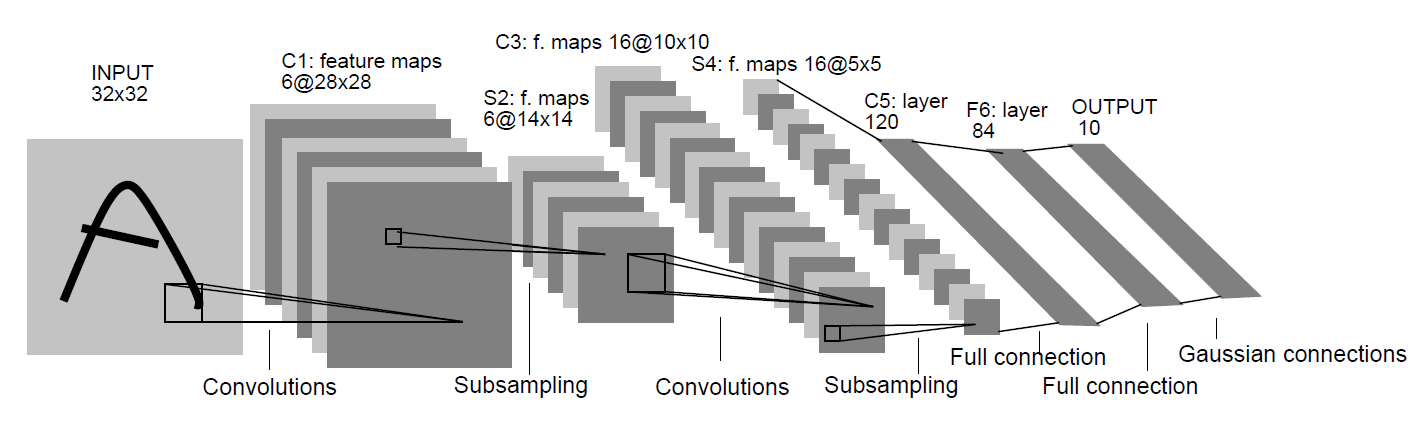
\includegraphics[width=8.3cm]{fig/Survey/LeNet5.png}
    \caption{Architecture of LeNet-5 the GreenEyes model.}
\end{figure}

LeNet-5 is a convolutional neural network (CNN), which is originally trained for digits recognition. Each plane is a feature map, which is an identical output from the last layer.

The simplest CNN, LeNet, established an era that models based on convolutional layers are widely used for various problems. For 2D image classification or recognition problems, there are VGG \cite{simonyan2014very}, ResNet \cite{he2016deep}, and so on. As for WaveNet, the convolution layers are 1-dimensional.

% \subsection{Other Kind of Neural Networks}

% \begin{figure}[!htbp]
%     \centering
%     \label{fig:Neural_Network_Zoo}
%     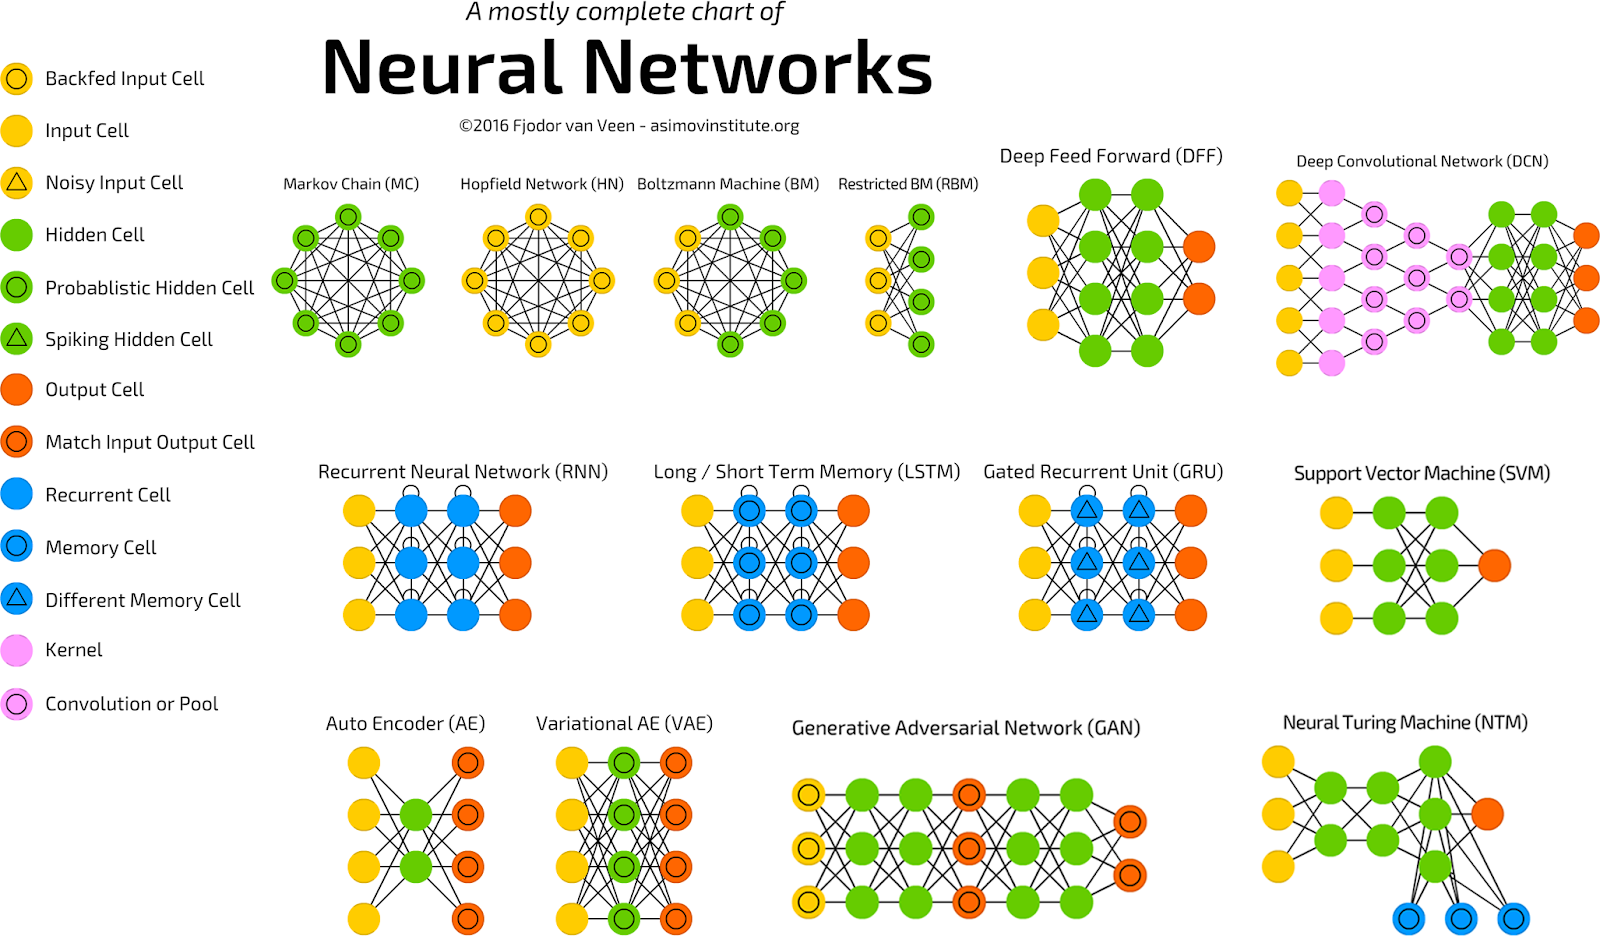
\includegraphics[width=8.3cm]{Survey/Neural Network Zoo (Courtesy of Asimov Institute).png}
%     \caption{}
% \end{figure}

% 按结构分,VAE等
% 任务,图像分类,物件识别,NLP

\subsection{Backpropagation and Optimization}

LeCun, etc \cite{lecun1998gradient} not only successfully built and trained a Neural Network but also brought forth a foundation method call gradient-based learning.

The two key elements of this method are the $loss$, and the $gradient$. Typically, $loss$ is a function of the prediction and the ground truth:

\begin{equation}
    L=f(y_{pred}, y_{truth})
\end{equation}

where $y_{pred}$ is the output of the model. Equations \ref{eq:gradient_equation} sums up common patterns of gradients.

\begin{eqnarray} \label{eq:gradient_equation}
    \frac{\partial E^p}{\partial W_n}=\frac{\partial F}{\partial W}(W_n,X_{n-1})\frac{\partial E^p}{\partial X_n} \nonumber \\
    \frac{\partial E^p}{\partial X_{n-1}}=\frac{\partial F}{\partial X}(W_n,X_{n-1})\frac{\partial E^p}{\partial X_n}
\end{eqnarray}

In a more recent review, LeCun \cite{hinton2015deep} also gave a visualization of gradients, as Figure \ref{fig:gradient_figure} shows. This figure also illustrates some relationships between brains and Neural Networks.

% TODO 要改
\begin{figure}[!htbp]
    \centering
    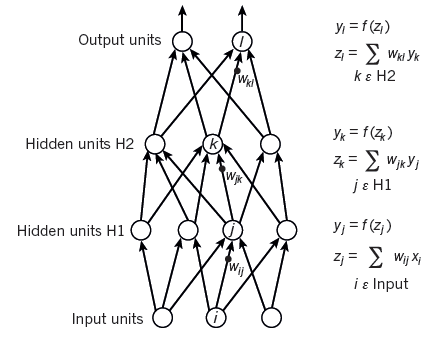
\includegraphics[width=2.9in]{fig/Survey/gradient_figure.png}
    \caption{Gradients in backpropagation between hidden layers.}
    \label{fig:gradient_figure}
\end{figure}

Nowadays, most NN frameworks such as PyTorch and TensorFlow support automatical computation for gradients. And with the GPU acceleration technics being widely used, we can train a model in a faster and more convenient way of computing these gradients.

\section{Components Used in Our Model}

Before interpreting our work of porting WaveNet into the application of time series fitting, we'll introduce several components for preliminaries.

\subsection{LSTM}

Sepp Hochreiter and Jürgen Schmidhuber \cite{hochreiter1997long} introduced "Long Short-Term Memory" (LSTM) to solve the gradient vanishing problem and gradient exploding problem.

\begin{figure}[!htbp]
    \centering
    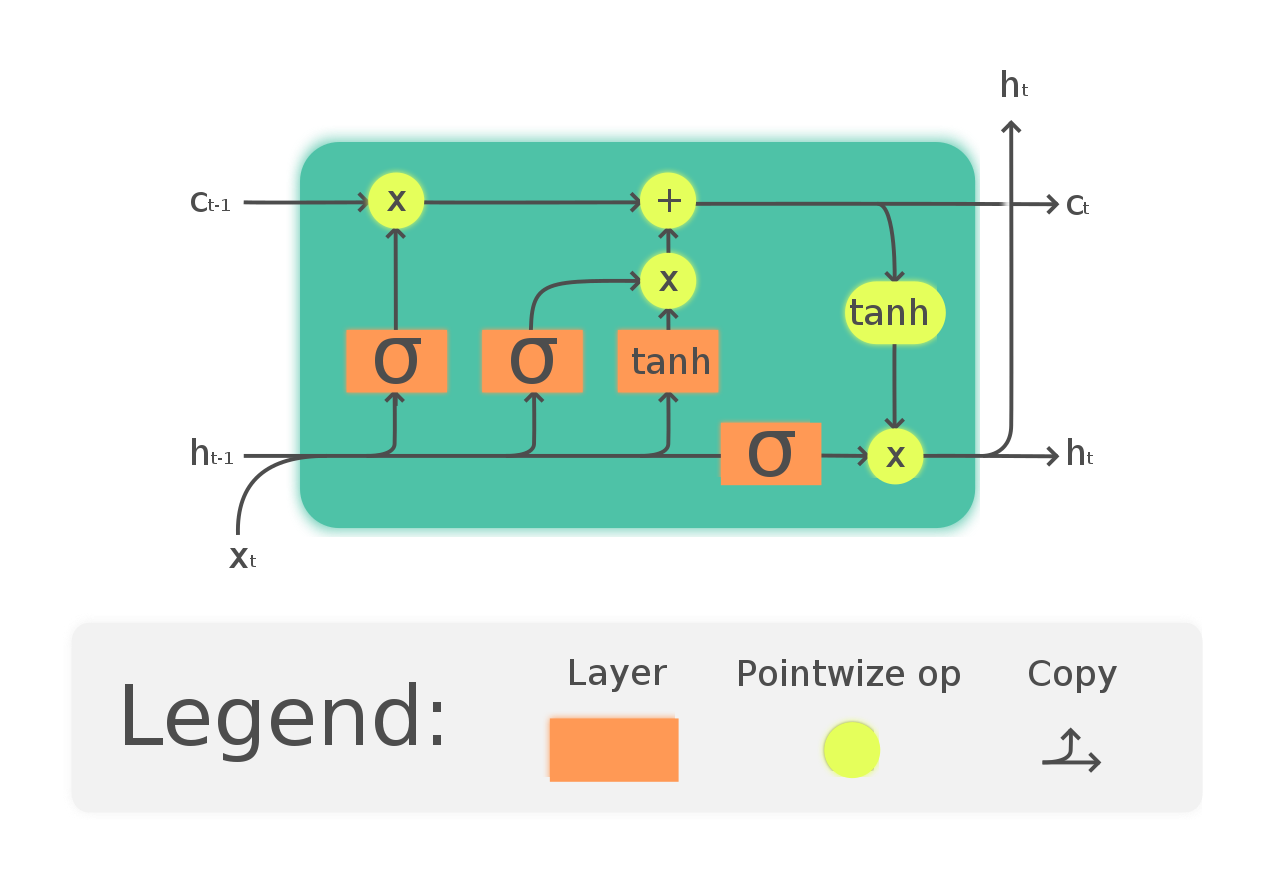
\includegraphics[width=8.3cm]{fig/Survey/The_LSTM_Cell.png}
    \caption{The Long Short-Term Memory (LSTM) cell can process data sequentially and keep its hidden state through time. \cite{wiki:LSTM}}
    \label{fig:The_LSTM_Cell}
\end{figure}

A common LSTM unit is composed of a cell, an input gate, an output gate, and a forget gate \cite{wiki:LSTM}. These gates give LSTM layers the feature of "memory"--remembering values over arbitrary time intervals.

LSTM can deal with Time Series Prediction, Natural language processing, and image processing tasks \cite{lindemann2021survey}.


\subsection{Attention}

Attention mechanism also came from NLP tasks and is also suitable for Time Series Fitting/Prediction problems.

\begin{figure}[!htbp]
    \centering
    \label{fig:luong-attention.png}
    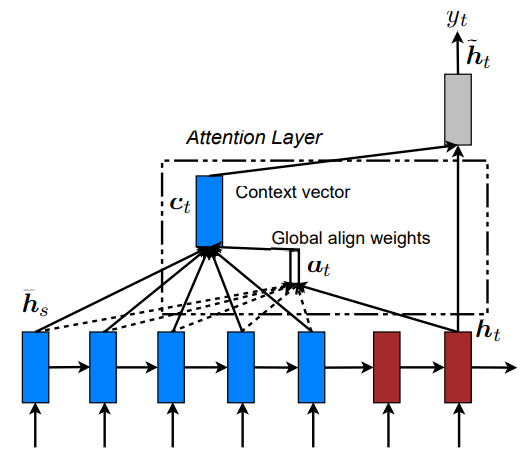
\includegraphics[width=8.3cm]{fig/Survey/luong-attention.png}
    \caption{Luong's \cite{luong2015effective} global attentional model.}
\end{figure}

Bahdanau \cite{bahdanau2014neural} Luong \cite{luong2015effective} respectively brought out additive style and multiplicative style attention.

The attention mechanism cam be formularized by following equations \ref{eq:attention_mechanism}, \ref{eq:attention_score}:

\begin{align} \label{eq:attention_mechanism}
    \alpha_{ts}&=\frac{exp(score({\textbf{\textit{h}}}_{t},\bar {\textbf{\textit{h}}}_{s}))} { \sum_{s'=1}^S exp(score({\textbf{\textit{h}}}_{t},\bar {\textbf{\textit{h}}}_{s'} )) } &\text{[Attention\ weights]} \\
    \textbf{\textit{c}}_{t}&=\sum_s \alpha_{ts} \bar {\textbf{\textit{h}}}_{s} &\text{[Context\ vector]} \\
    \textbf{\textit{a}}_{t}&=f(\textbf{\textit{c}}_{t},\textbf{\textit{h}}_{t})=tanh({\textbf{\textit{W}}}_{\textbf{\textit{c}}} [\textbf{\textit{c}}_{t};\textbf{\textit{h}}_{t}]) &\text{[Attention\ vector]}
\end{align}

\begin{equation} \label{eq:attention_score}
    score({\textbf{\textit{h}}}_{t},\bar {\textbf{\textit{h}}}_{s}) = \left\{
    \begin{array}{lr}
    {\textbf{\textit{h}}}_{t}^\top\textbf{\textit{W}}\bar {\textbf{\textit{h}}}_{s} & {\text{[Luong's multiplicative style]}} \\
    \textbf{\textit{v}}_{a}^\top tanh({\textbf{\textit{W}}}_\textbf{1}{\textbf{\textit{h}}}_{t}+{\textbf{\textit{W}}}_\textbf{2}\bar {\textbf{\textit{h}}}_{s}) & {\text{[Bahdanau's additive style]}}
    \end{array}
    \right.
\end{equation}

Attention mechanism gives models the capability of paying attention to a part of the data by attention weights.
